% begin module tangents-reminder
\begin{frame}
\frametitle{Tangents}
\begin{center}
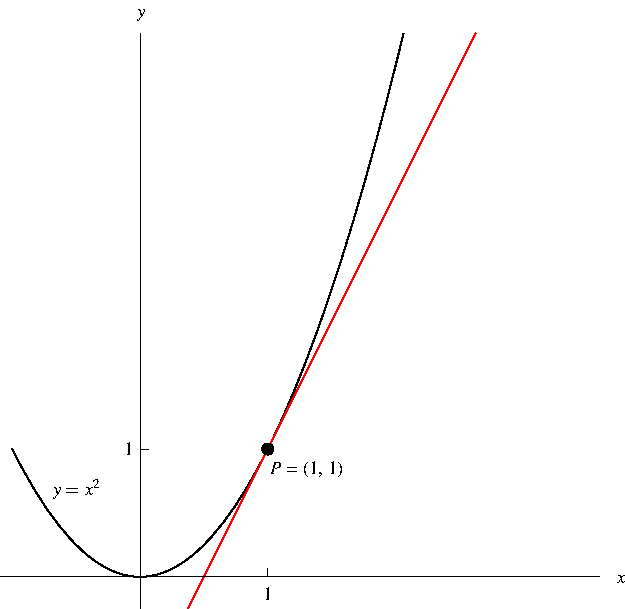
\includegraphics[height=5cm]{derivatives/pictures/02-01-secanta.pdf}%
\end{center}
\begin{itemize}
\item<2->  Recall that in section (2.1) we tried to find the tangent line to the curve $y = x^2$ at the point $P = (1,1)$.
\item<3->  This problem motivated us to study limits.
\end{itemize}
\end{frame}


\begin{frame}
\begin{columns}[c]
\column{.4\textwidth}
\ \only<handout:0| -1,11->{%
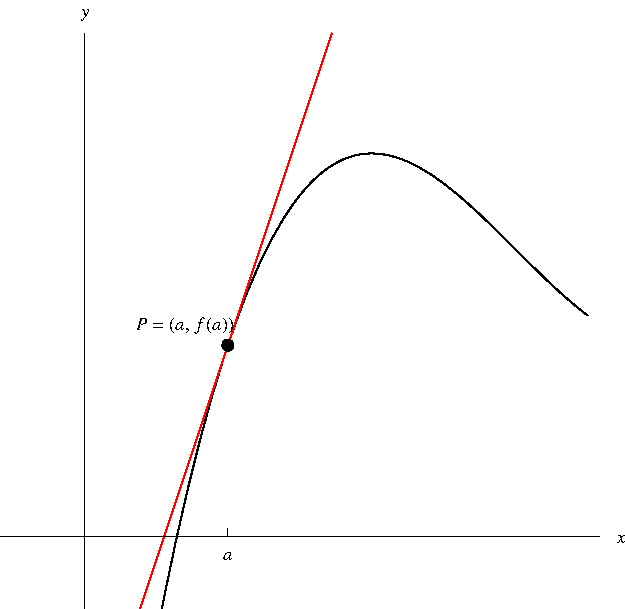
\includegraphics[height=4.5cm]{derivatives/pictures/03-01-tangent.pdf}%
}%
\only<2-4>{%
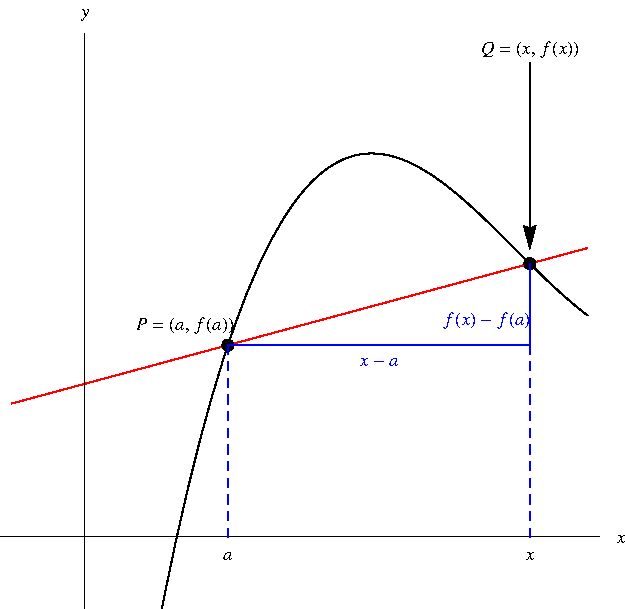
\includegraphics[height=4.5cm]{derivatives/pictures/03-01-secanta.pdf}%
}%
\only<handout:0| 5>{%
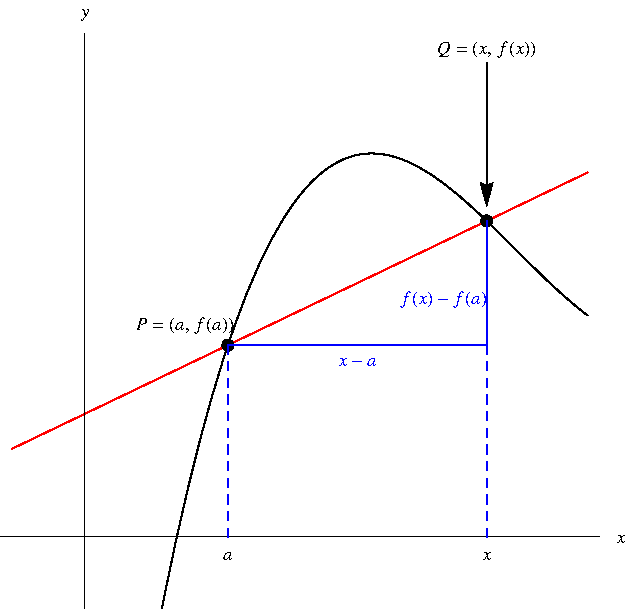
\includegraphics[height=4.5cm]{derivatives/pictures/03-01-secantb.pdf}%
}%
\only<handout:0| 6>{%
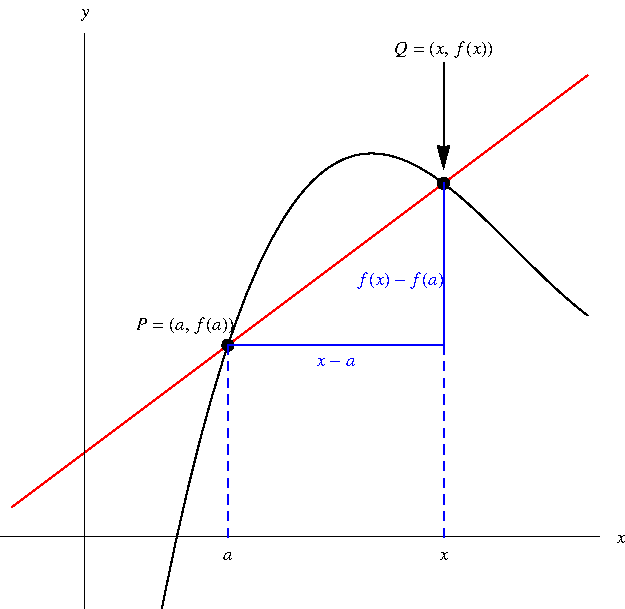
\includegraphics[height=4.5cm]{derivatives/pictures/03-01-secantc.pdf}%
}%
\only<handout:0| 7>{%
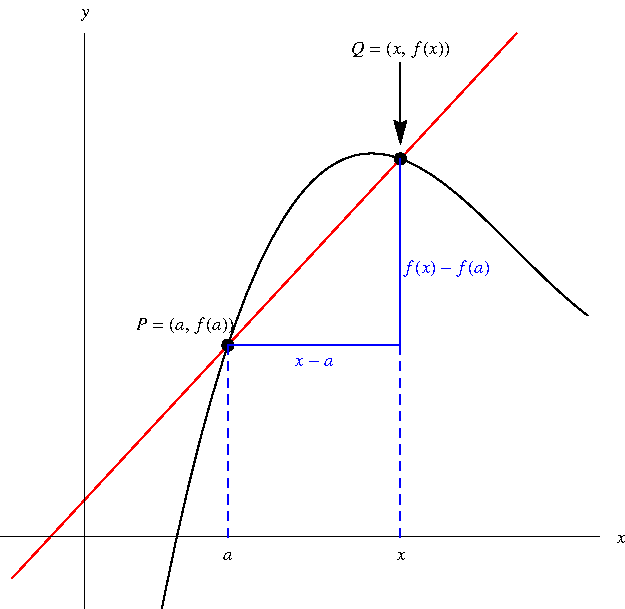
\includegraphics[height=4.5cm]{derivatives/pictures/03-01-secantd.pdf}%
}%
\only<handout:0| 8>{%
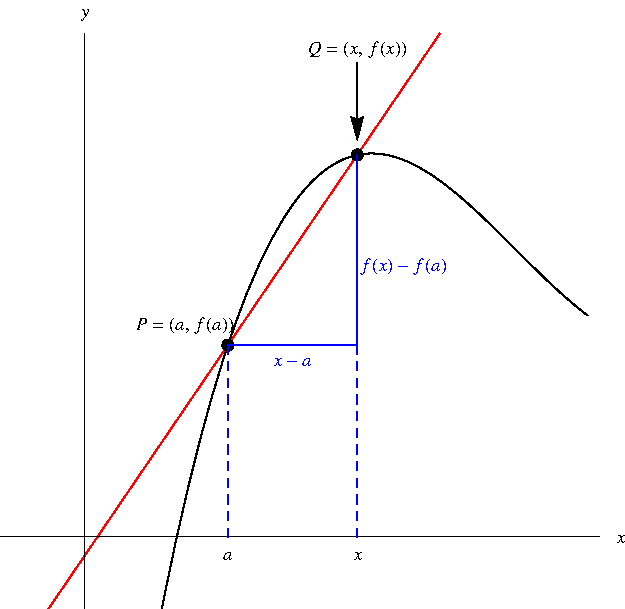
\includegraphics[height=4.5cm]{derivatives/pictures/03-01-secante.pdf}%
}%
\only<handout:0| 9>{%
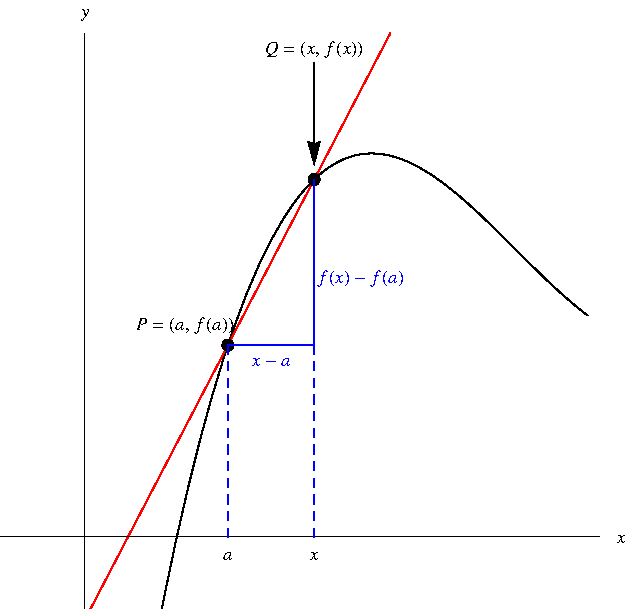
\includegraphics[height=4.5cm]{derivatives/pictures/03-01-secantf.pdf}%
}%
\only<handout:0| 10>{%
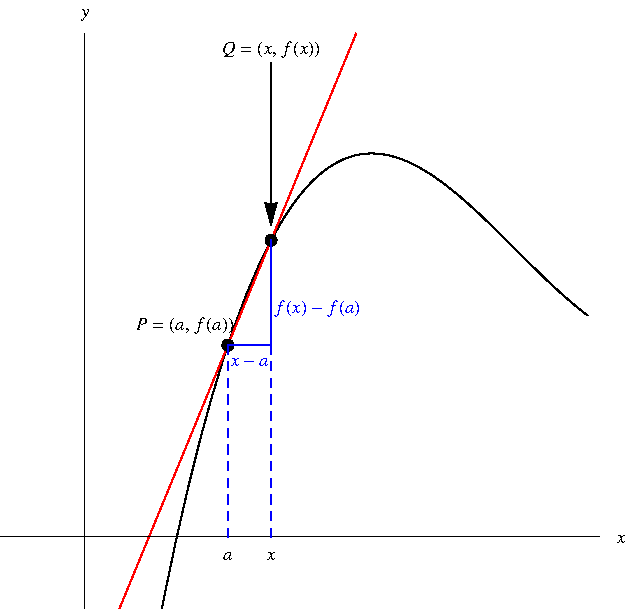
\includegraphics[height=4.5cm]{derivatives/pictures/03-01-secantg.pdf}%
}%
\column{.6\textwidth}
\begin{itemize}
\item<1->  How to find the tangent line to the curve $y = f(x)$ at $P = (a, f(a))$?
\item<2->  Consider a nearby point $Q = (x, f(x))$.
\item<3->  Compute slope of secant line $PQ$: $m_{PQ} = \frac{f(x)-f(a)}{x-a}$.
\item<4->  Let $Q$ approach $P$ along the curve by letting $x$ approach $a$.
\end{itemize}
\end{columns}
\uncover<11->{%
\begin{definition}[Tangent Line]
The tangent line to the curve $y = f(x)$ at the point $P = (a, f(a))$ is the line through $P$ with slope
\[
m = \lim_{x\rightarrow a}\frac{f(x) - f(a)}{x-a}
\]
provided that the limit exists.
\end{definition}
}%
\end{frame}
% end module tangents-reminder
